\begin{EXO}{Tableau de signes avec forme canonique}{}
Soit $f$ une fonction définie sur $\R$ par $f(x) = -2(x-5)^2+13$. 

\tcbitempoint{3} Dresser le tableau de signes de $f$.

\begin{crep}
Racines : $f(x) = 0 \Rightarrow (x-5)^2 = \dfrac{13}{2}$\hfill D'où $x = 5 \pm \sqrt{\dfrac{13}{2}}$\hfill\phantom{a}\\\\
\begin{center}
\begin{tikzpicture}
\tkzTabInit{$x$/1,$f(x)$/1}
{$-\infty$,$5-\sqrt{\frac{13}{2}}$,$5+\sqrt{\frac{13}{2}}$,$+\infty$}
\tkzTabLine{,-,z,+,z,-}
\end{tikzpicture}
\end{center}
\end{crep}

\exocorrection

$f(x) = -2(x-5)^2+13$ est sous forme canonique avec $a = -2 < 0$.

Pour trouver les racines, résolvons $f(x) = 0$ :

$-2(x-5)^2+13 = 0 \Rightarrow (x-5)^2 = \dfrac{13}{2}$

$x-5 = \pm\sqrt{\dfrac{13}{2}} \Rightarrow x = 5 \pm \sqrt{\dfrac{13}{2}}$

Comme $a = -2 < 0$, la parabole est tournée vers le bas.

$f(x) > 0$ entre les racines et $f(x) < 0$ à l'extérieur.
\end{EXO}